\documentclass[12pt]{article}

\usepackage[english]{babel}
\usepackage[utf8x]{inputenc}
\usepackage{amsmath}
\usepackage{graphicx}
\usepackage{longtable}
\usepackage{hyperref}
\usepackage{natbib}

\usepackage{comment}
\includecomment{todo}
%\excludecomment{changelog}
%\excludecomment{todo}

\newcommand\x         {\hbox{$\times$}}
\newcommand\othername {\hbox{$\dots$}}
\def\eq#1{\begin{equation} #1 \end{equation}}
\def\eqarray#1{\begin{eqnarray} #1 \end{eqnarray}}
\def\eqarraylet#1{\begin{mathletters}\begin{eqnarray} #1
                  \end{eqnarray}\end{mathletters}}
\def\mic              {\hbox{$\mu{\rm m}$}}
\def\about            {\hbox{$\sim$}}
\def\Mo               {\hbox{$M_{\odot}$}}
\def\Lo               {\hbox{$L_{\odot}$}}
\def\comm#1           {{\tt (COMMENT: #1)}}
\def\kms   {\hbox{km s$^{-1}$}}

\usepackage[usenames]{color} 
\newcommand{\G}[1]{{\color{red} #1}}
\newcommand{\B}[1]{{#1}}
\newcommand{\R}[1]{{\color{red}}}
\newcommand{\code}[1]{\texttt{#1}}



\title{Hyper Suprime-Cam Survey \\
  Pipeline Description}
\author{
  The HSC Pipeline Team: \\
  Hisanori Furusawa,
  Michitaro Koike,
  Yuki Okura, \\
  Tadafumi Takata,
  Yoshihiko Yamada (NAOJ Mitaka), \\
  Naoki Yasuda,
  Steve Bickerton,
  Sogo Mineo (IPMU), \\
  Robert Lupton,
  Jim Bosch,
  Craig Loomis, \\
  Hironao Miyatake,
  Paul Price (Princeton) \\
}


\begin{document}
\maketitle
\pagestyle{headings}

\begin{abstract}
\end{abstract}

\clearpage

\tableofcontents

\clearpage

\section{Introduction}

This document describes the Hyper Suprime-Cam Survey Pipeline, which will be used to process the survey
observations and deliver data products with a consistent high quality to the collaboration, and ultimately to
the world, for the realisation of the survey science goals.

\subsection{Hyper Suprime-Cam}

%%%
%%% Stolen from the proposal, with some edits
%%%

Hyper Suprime-Cam takes advantage of the full accessible field of view of the Subaru telescope (1.5~deg$^2$
diameter).  The focal plane is paved with 104 Hamamatsu Deep Depletion science CCDs (plus another 8 guiding
and wavefront monitoring CCDs), each 2k\x 4k. These chips, which are three-side buttable and each have four
independent readout amplifiers, are currently installed in Suprime-Cam, which has demonstrated their excellent
characteristics: low read noise, excellent charge transfer efficiency, few cosmetic defects, and most
importantly, high quantum efficiency from 4000\AA\ to 10,000\AA.  The CCD pixels are $15\mu$m on a side,
corresponding to $0.16$~arcsec at the focal plane. At this resolution, the images will be well-sampled in even
the best seeing.  Ray-tracing of the optics has shown that ghosting is minimal, with the worst ghost at an
illuminance (fractional light in a PSF aperture) of $\sim 5 \times 10^{-8}$.

Details of the instrument are summarized in the Hyper Suprime-Cam
Design Review
Booklet\footnote{\url{http://anela.mtk.nao.ac.jp/hypersuprime/presentation/hscreview20090227final_combined.pdf}}. The
official HSC
webpage\footnote{\url{http://www.naoj.org/Projects/HSC/index.html}}
provides up-to-date information.

\subsection{The HSC Survey}

%%%
%%% Stolen from the proposal, with edits
%%%

The HSC Survey was initiated to address key scientific questions using the new capabilities afforded by HSC.
The principal science drivers are:
\begin{itemize}
\item Studies of the properties of dark matter and dark energy as a
  function of redshift, using measurements of galaxy clustering, weak
  lensing, supernovae, cross-correlation with high-resolution maps
  of the Cosmic Microwave Background, and studies of high-redshift
  quasars.
\item Studies of the evolution of galaxies over cosmic time, with
  emphasis on stellar populations and star formation, morphologies, and
  active nuclei.
\end{itemize}

The survey has a classical ``wedding cake'' design, with three layers.  The Wide layer will cover roughly
1,400~deg$^2$ in five broad filters ($grizy$), with exposure times of $10-20$~min per pointing (and one with a
shorter exposure time of $\sim 30$~sec to enable astrometric and photometric calibration with other surveys).
This will go to a point-source depth of $r\sim 26$, and is optimized for weak-lensing science.  Using galaxies
for weak lensing will require exquisite understanding of their properties and evolution, which will be the
motivation of the Deep layer, covering 27~deg$^2$ in four distinct fields, going roughly one magnitude deeper
with exposures of roughly 1~hr per filter.  In addition to the broad-band filters, the Deep layer will include
imaging in three narrow-band filters, to detect Lyman-$\alpha$ emitters and study their luminosity function
and clustering properties at $z = 2.2$, 5.7, and 6.6.

To study the faintest and most distant galaxies, and to probe the
transient universe, especially high-redshift supernovae, will require
the Ultradeep layer, going another magnitude fainter yet.  Narrow-band
filters in the Ultradeep layer will search for Lyman-$\alpha$
emitters at $z = 5.7$, 6.6, and 7.3 at the very faint end of the
luminosity function.

\subsection{This document}

This document provides a reference to the HSC Pipeline which will be
used to process the HSC Survey observations, producing the necessary
data to achieve the scientific goals of the survey.  It is
especially intended for HSC Survey scientists to evaluate the pipeline
and its products in relation to their own science goals.

In section \ref{sec:pipeline}, we outline the pipeline construction and operations, tracing the flow of data
through the various stages of the pipeline, to the ultimate releases to the collaboration.  Next, in section
\ref{sec:products}, we outline the various products that will compose the data releases, with particular
attention to the measurements that comprise the catalog in the database.  Section \ref{sec:algorithms} gives
details as to the algorithms used to make these measurements, and section \ref{sec:interfaces} describes how
the data will be made available.  Finally, section \ref{sec:support} contains pointers on resources available
for supporting users of these data.


\section{The HSC Pipeline}
\label{sec:pipeline}
\subsection{Software}

%%%
%%% Stolen from the proposal
%%%

To construct the HSC pipeline, we use the LSST pipeline software as the foundation.  This is a synergistic
effort, since the pipelines have similar functionality.  By this scheme, the HSC pipeline has features and a
maturity it would not otherwise have at this stage, and because our pipeline is based on code with a larger
market share than ours could ever have alone, we can have greater confidence in the results.  In return, LSST
gains testing and verification with real-world data.  However, since LSST is a larger-scale development
project not entirely within our control, we are selective about the LSST components we use for the HSC
pipeline, so that we are not chained to every design decision of LSST.  We have also supplemented LSST
components with different algorithms, and added new pipeline components as necessary.  The LSST code is
released under the GNU Public License, version 3 (or later), and our releases of our modified versions of that
code, and our own code (as a ``derivative work'') are bound to use the same license.

The pipeline is written in Python, using C++ for low-level algorithmic components where speed is important.
SWIG is used to wrap the C++ components so they can be called directly from Python.  The combination of these
results in all the ease and flexibility of a scripting language while retaining the power of a compiled
language.

Particular attention has been paid, in large part because of our contributions, to making the LSST pipeline
extensible and configurable.  New camera interfaces and new measurement algorithms can be added without the
need to redesign or even rebuild the software.  The modular design also allows for algorithms to be
substituted at run-time, so that the pipeline can adapt to the data being processed.  These features, besides
being useful for our adaptation of the LSST pipeline to HSC, mean that we could use our own pipeline to
process data from other telescopes and cameras for comparison with the results of other pipelines (e.g., we
can not only compare the results of the HSC Survey + HSC pipeline with DECam + DES pipeline, but also with
DECam + HSC pipeline, for better diagnosis of any problems).  Interface packages have been written for LSST
simulated images (``ImSim''), CFHT MegaCam, Subaru's Suprime-Cam, SDSS, the Space Surveillance Telescope
(SST), DECam, and HSC simulated images.

Testing with archival Suprime-Cam data (in particular, from after August 2008 when the Hamamatsu CCDs were
installed) and more recently with HSC commissioning data has been an integral part of the pipeline development.

\subsection{Data flow}

The pipeline consists of multiple stages in order to produce the variety of data products required to meet the
various survey science goals.  The stages share a great deal of framework code, but differ by their inputs,
parallelism scheme (CCD vs exposure vs sky patch) and outputs.  Different science applications will depend on
different pipeline stages, according to the desired measurements, depth and accuracy.

\begin{figure}[!htbp]
    \centering
    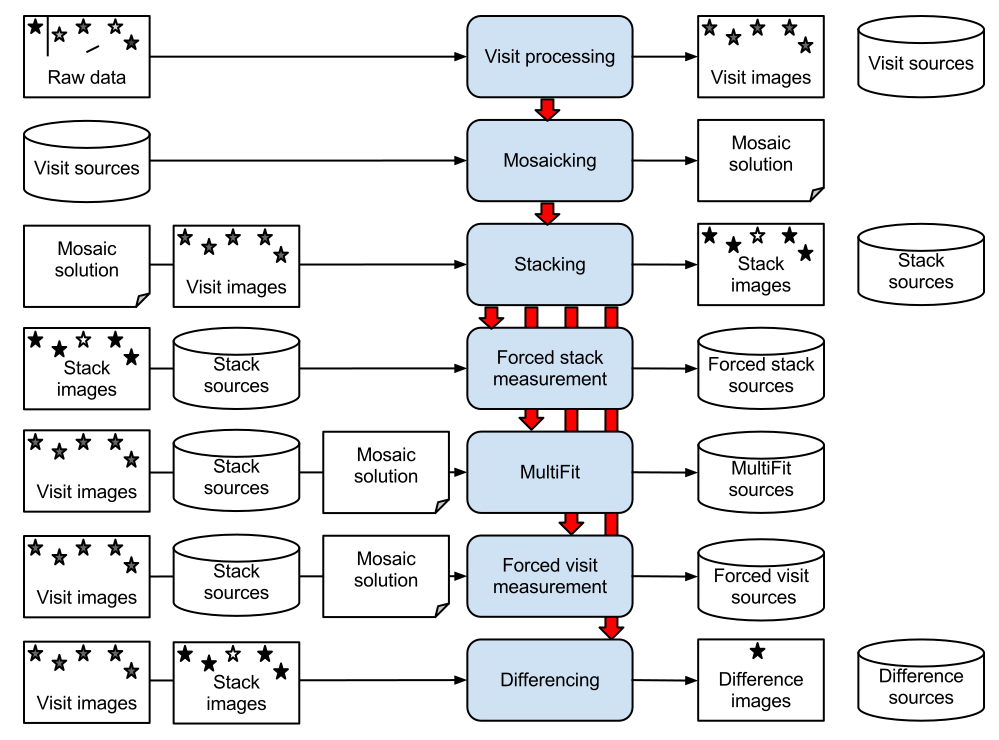
\includegraphics[scale=0.5]{figures/HSCpipelinesketch}
    \caption{HSC Pipeline data flow\label{fig:flow}}
\end{figure}

Figure~\ref{fig:flow} shows a schematic representation of the HSC pipeline.  Input data on the left is fed
into the pipeline stages (light blue, center) to produce the outputs on the right.  The first three stages
(visit processing, mosaic solution, stacking) are executed in sequence, after which all the remaining stages
can be run in parallel.  The stages are explained in more detail below.

\subsubsection{Visit processing}

Visit processing removes the instrumental signature (overscan, bias, dark, flat, bad pixels, amplifier
crosstalk) from each CCD and flags suspected cosmic-rays.  The result is a clean image for which the intensity
is a linear function of astrophysical flux\footnote{Excepting flat-field inaccuracies, and intrinsic pixel
  shape non-linearities.}  The background is estimated and removed, then bright sources on the image are used
to measure the PSF and the astrometric solution and photometric zero-point, before a final detection and
measurement pass.  From the individual CCD measurements, we determine and apply an exposure-wide astrometric
solution and photometric zero-point.

The ouputs are:
\begin{itemize}
\item Image
\item PSF
\item Background
\item Sources
\item Astrometric solution
\item Photometric zero point
\end{itemize}

\subsubsection{Mosaic solution}

Once several exposures overlapping the same part of sky are available, we can determine a mosaic solution.
This involves solving for consistent astrometric solutions and photometric zero-points for the set of
exposures, using sources in common to multiple exposures, in the same manner as \citet{2008ApJ...674.1217P}.
This allows increased accuracy and precision relative to the visit processing, by allowing use of stars
fainter than in our original reference catalog (e.g., SDSS), and incorporating spatial information unavailable
from single exposures.


\subsubsection{Stacking}




\subsubsection{Forced Stack Measurement}
\subsubsection{MultiFit}
\subsubsection{Forced Visit Measurement}
\subsubsection{Differencing}
\subsection{Releases}
\subsubsection{Daily}
\subsubsection{Monthly}
\subsubsection{Semi-annually}

\section{Data Products}
\label{sec:products}
\subsection{Images}
\subsubsection{Visits}
\subsubsection{Stacks}
\subsubsection{Differences}
\subsection{Catalogs}
\subsubsection{Visits}
\subsubsection{Stacks}
\subsubsection{Forced Visit Measurements}
\subsubsection{Forced Stack Measurements}
\subsubsection{MultiFit}
\subsubsection{Differences}
\subsection{Database}
\subsubsection{Schema}

\section{Algorithms}
\label{sec:algorithms}
\subsection{Flags}
\subsection{Measurements}
\subsection{Background Matching}
\subsection{CoaddPsf}
\subsection{Skymap}

The ``skymap'' is a tessellation of the sky, providing suitable pre-defined coordinate systems for operations
on the sky such as stacking.  The sky map divides the sky into ``tracts''.  For convenience and parallelism,
each tract is sub-divided into ``patches''.  Tracts and patches overlap, so that sources are not lost in the
gaps.  These overlaps can be both annoying (additional care is required to remove duplicate sources) and
useful (additional source of quality checking).

Our tracts tangent planes (\code{TAN} WCS) distributed in rings of Declination, which matches well with the
survey geometry.  This has more inefficiency (tract overlap) at the pole, but since our survey doesn't cover
that area, it's not a problem.  Individual tracts are roughly the same size as the field of view of HSC, and
have North and East vectors aligned with the columns and rows, respectively.

\begin{figure}[!htbp]
    \centering
    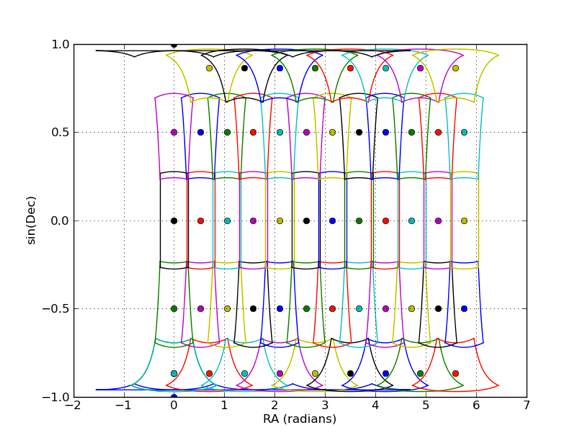
\includegraphics[scale=0.3]{figures/rings_equat.png}
    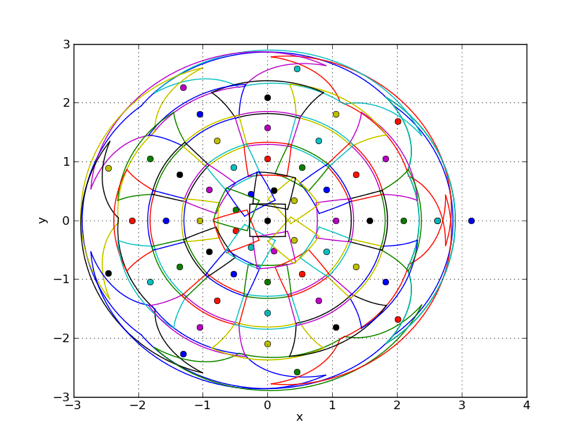
\includegraphics[scale=0.3]{figures/rings_pole.png}
    \caption{Demonstration of the skymap scheme we will use for the HSC pipeline.  Left: Equatorial
      projection.  Right: Polar projection.  Note that the tracts shown here are very much larger than we will
      use in practise; the large tracts allows the characteristics of the tessellation (e.g., the larger
      overlap at the poles) to be more clearly discerned.\label{fig:skymap}}
\end{figure}

\subsection{Mosaic}

\section{External Interfaces}
\label{sec:interfaces}
\subsection{Database}
\subsection{Postage Stamps}
\subsection{Copying}

\section{Help and Support}
\label{sec:support}
\subsection{Forum}
\subsection{Mailing list}

\clearpage

\bibliographystyle{}
\bibliography{pipeline/pipeline}

\begin{todo}
\clearpage
\section{TODO}
\begin{itemize}
\item Nothing yet.
\end{itemize}
\end{todo}

\end{document}
